% Subsection 4.1: imageSubtraction

\subsection{Image Subtraction}
\label{ImageSubtraction}\label{sApp-imsub}

The essence of Image Subtraction is to design a convolution
\code{Kernel} $K$ that  photometrically registers the
point-spread functions (PSFs) of two images.  One image is (ideally)
an essentially noiseless and defect-free template image $T$ created through
coaddition of many individual science images.  The other is the
science image $I$ obtained on a given night.  After registration,
subtraction of the template image from the science image should yield
a difference image $D$ that contains only those things that have
varied in position or brightness from the template.

Since this process involves the convolution of an image, for DC2 we
decided that we will \textit{always} build the \code{Kernel} to operate
on the template image, leaving the science pixels untouched.  The
advantages of this are two-fold: since convolution is
expected to be a smoothing process, you can afford to correlate the
pixels in the template image more than you can in the science image
since they are less noisy; and since the template is assumed to be
defect-free, we can minimize the effect that convolution spreads the
influence of bad pixels.  

The creation of $D$ is a fundamental role of LSST's nightly pipeline.
This image will feed the nightly alert stream, which will be the public face
of LSST for many scientists.  It's important we get this part of the
reductions right, which is why we began development of this stage in
DC2, with large lead time to first light.

\subsubsection{Key Framework Classes}

Image Subtraction required design and development of several key
Framework and Detection classes.  The key Framework classes developed
during the course of DC2, and how they were used, are listed below.

\begin{itemize}
\item \code{lsst::fw::Exposure} ---
   Input images from the CFHT were read into \code{Exposures}, a
   combination of a \code{MaskedImage} and its associated \code{WCS}.
   The template and science image \code{MaskedImages} were the
   fundamental objects being passed between the Image Subtraction
   stages.

\item \code{lsst::fw::Kernel} ---
   Three sets of convolution \code{Kernel}s were created in the DC2
   implementation of Image Subtraction.  They were used to match the
   PSFs of the two images in different \code{Footprint}s.  A spatial
   model was also built using the \code{Function} class below.

\item \code{lsst::fw::function::Function} ---
   This allows the user to create one or two-dimensionally spatially
   varying functions.  DC2 used \code{Functions} to represent the
   final spatially varying Image Subtraction \code{Kernel}, as well as
   a spatially varying differential background correction.

\item \code{lsst::fw::function::MinimizerFunctionBase} ---
   This internal class allows the user to fit for the coefficients of
   a \code{Function} using \code{lsst::fw::function::minimize}, \
   given a set of input constraints.  
   \code{MINUIT}\footnote{http://www.cern.ch/minuit} was used for
   the non-linear fitting backend.

\item \code{lsst::imageproc::DiffImContainer} ---
   A \code{DiffImContainer} was created for each \code{Footprint} used
   to constrain the \code{Kernel} model.  It holds pointers to the
   different versions of \code{Kernel}s that were built, summary
   statistics on the associated difference images, the background
   measurement at its position, and if the \code{Footprint} has passed
   or failed goodness-of-fit criteria.

\end{itemize}

\subsubsection{The Algorithm}

Image Subtraction is implemented using a combination of controlling
Python scripts and number-crunching C++ code.  To
create a useful reference for future designers, we will distinguish
which operations are implemented in which language.

The first stage is implemented in Python.  It reads the CFHT
template and science images from disk, and turns them into two
\code{MaskedImages}.  It also reads in the \code{Policy} file that
controls e.g.~the \code{Kernel} sizes, how large to make the
\code{Footprint}s, how faint one should go when searching for these
\code{Footprint}s, and the criteria used to reject bad
\code{Footprint}s during the \code{Kernel} creation process.

The Python code then calls the C++ routine
\code{getCollectionOfFootprintsForPsfMatching}.  This in turn calls 
the \code{Detection} code to search for significant peaks above
background in the Template image.  For reduction of commissioning
data, we will likely have to operate in this mode.  However, for
subsequent operations we should be able to query the Database for the
locations of appropriate positions.  These are returned as a list of
\code{Footprint}s.  Each \code{Footprint} is then searched for 
masked pixels in both the Template and Science images.  Any masked
pixels in the \code{Footprint} causes it to be rejected.  They are
then grown by a certain amount specified in the \code{Policy}, and
returned to the controlling Python script to have PSF-matching
\code{Kernel}s built for each one.

For each returned \code{Footprint}, a \code{DiffImContainer} is
created in Python, and the first \code{Kernel} is created.  The
C++ routine \code{computePsfMatchingKernelForPostageStamp} \
generates \code{Kernel} Model I for a given \code{Footprint}.  This
uses a delta-function set of basis functions to create the most
general \code{Kernel} possible.  The associated difference image is
examined, and the \code{Footprint} is rejected if the residuals are
too large (``too large'' having been defined in the input
\code{Policy}).  The outputs are a single \code{Kernel} and a DC
differential background correction between the template and science
image.

In Python, the \code{Kernel}s are examined as an ensemble.  In
particular, the distribution of the \code{Kernel}s sums (the
photometric rescaling, or the \code{Kernel}s ``volume'') is examined
and outliers are rejected.  These outliers might be e.g.~variable
stars.

Next the C++ function \code{computePcaKernelBasis} is called.
The inputs are the ensemble of good \code{Kernel}s.  This routine runs
a Principal Component Analysis (PCA) on the ensemble, creating an
orthonormal basis set of eigen-\code{Kernel}s from the data
themselves.  The hope is that the input \code{Kernel}s are
similar enough to justify approximating each one with a compact
set of eigen-\code{Kernel}s.  The number of eigen-\code{Kernel}s
chosen was defined in the \code{Policy}, and for DC2 was a minimum of
3, and enough to account for 95\% of the variance, up to a maximum
of 7.
%
Each input \code{Kernel} is approximated by deriving the coefficient
in front of each eigen-\code{Kernel} through their dot product, a
process that yields \code{Kernel} Model II, a PCA approximation of
each input \code{Kernel}.  The associated difference image is
examined, and the \code{Footprint} is rejected if the residuals are
too large.  If any are rejected, the PCA is re-run, until this
process converges.

Finally, the Python code calls the C++ routine
\code{computeSpatiallyVaryingPsfMatchingKernel}, which fits 
spatially varying \code{Functions} to the eigen-\code{Kernel}
coefficients (yielding \code{Kernel} Model III) as well as a spatially
varying background.  The spatial orders are specified in the input
\code{Policy}.  This allows a \code{Kernel} to be generated for, and
applied to, each pixel in the input images, allowing creation of the
difference image.  The difference image is persisted as a
\code{MaskedImage} and the \code{Kernel} and background as
\code{Functions}.

\subsubsection{Performance}
\label{ImageSubtraction-Performance}

For DC2, the \code{Kernel} Model I was very successful.  The mean
residual (normalized by the noise) across all \code{Footprint}s was
0.00, while the variance of this distribution was 1.06.  The final
variance is derived from the quadrature sum of the science image's
variance and the template image's variance (assumed to be zero for
DC2) convolved with the square of the \code{Kernel} values.  We find
that much of the extra noise came from \code{Footprint}s which should
have been masked but were not, due to e.g.~unrecognized saturated
stars.  Ideally, these \code{Footprint}s would have been skipped had
we had access to the imaging data from the start.  However,
significant pre-processing was done by the CFHT team and we were not
able to determine exactly which pixels had been saturated.
\code{Kernel} steps II and III were executed in DC2 with effectively
no sigma clipping of the input \code{Kernel}s.  This led to a success
rate of 98.7\% on the input CFHT images, with the remaining 1.3\%
having an anomalously large number of
detections per difference image.  This is commensurate with the
success rate for modern difference imaging pipelines.

The egregious failures (1.3\% of the input data) had two origins.  The
first were misregistrations of the input data, which was
out-of-scope for DC2 but will be in-scope for DC3.  These may be
recognized due to the very small ($\sim 0.0$) \code{Kernel} sums, as
the code tries to take an object in the template and match it to the
science image, which in general has no signal at that position.  The
second was a true failure of the pipeline.  These difference images had
\textit{very} strong gradients in the background, and significant
spatially varying residuals around the positions of objects.  This was
traced back to the sigma clipping processes: in these cases, the cuts
were too severe and rejected all but a few \code{Kernel}s.  These 2--3
\code{Kernel}s were then used to fit a spatially varying function,
which was effectively underconstrained.  This suggests that the sigma
clipping algorithms need to be more intelligent, and that there should
be some intelligence (perhaps in the \code{Function} classes) as to if
there are enough constraints to fit for a given order \code{Function},
which would increase or decrease the order of the \code{Function}
accordingly.  Care should also be taken to ensure that there are
constraints at the extremes of where the \code{Functions} will be
evaluated, in particular at the corners of the images.

As a research addendum to DC2, we created a ticket (\ticket{286}) that further
investigated the \code{Kernel} fitting process.  We added additional
steps of quality assurance and logging.  We found that when sigma
clipping was turned on for \code{Kernel} steps II and III, we were
sometimes losing too much information in the PCA step (II).  The sigma clipping
process would remove nearly \textit{all} \code{Kernel}s.  A closer
investigation revealed that these input science images had a PSF smaller
than the template image.  This meant that the \code{Kernel}s that were
built to match the template PSF to the science image PSF ended up
being \textit{deconvolution} \code{Kernel}s.  For these runs, the
ensemble of deconvolution \code{Kernel}s was not similar enough
to be accurately modeled by a small number of eigen-\code{Kernel}s.
This significantly impacted the final quality of the output difference
images.  This is likely the cause of the low-level dipole residuals
seen in the DC2 difference images.

\subsubsection{Convolution vs. Deconvolution}

This realization led to an investigation of the merits of convolving a
noisy science image versus deconvolving a template image.  There are
two competing issues here.  First is that we wish to ``convolve'' or
``smooth'' the image with the better PSF; deconvolution or sharpening
tends to increase high frequency noise and is not recommended for
anything but the highest signal-to-noise (S/N) data.  The second is
that we we wish to operate on the template image; it will have higher
S/N than the science images and should be relatively defect-free,
avoiding the spreading of bad pixels into adjacent pixels that happens
during convolution.  However, for DC2 we came across the situation
where the template image had worse seeing than the science image,
requiring we either deconvolve the template image or convolve the
science image.   This situation will also arise for LSST, particularly
early in the survey.

\Fig{fig-conv} illustrates this issue.  Each row shows, from
left to right: the image that was operated on; the image that it was
matched to; the derived convolution \code{Kernel}; and the final
difference image.  For the top row, the image that was operated on was
the science image (its apparent that the background is more noisy),
and it was matched to the template image.  The PSF of the science
image is smaller than the PSF of the template image, meaning the
\code{Kernel} \textit{convolved} or smoothed the science image.  The
\code{Kernel} indeed looks like a smoothing \code{Kernel}, compact and 
with most of its power in the center.  However, convolving the noisy
science image has generated correlated noise in the difference image;
 in general the
output noise will be increased when smoothing a noisy input
image.

For the bottom row, the image that was operated on was the template
image (it's apparent that the background is very smooth), and it was
matched to the science image.  The \code{Kernel} has high-frequency
power, as you would expect from a \textit{deconvolution}
\code{Kernel}.  The difference image has apparently uncorrelated 
noise, and is ideally what one expects from an output difference
image.  However, we determined during DC2 that we were unable to
compactly model an ensemble of deconvolution \code{Kernel}s using this
PCA technique --- the different \code{Kernel}s were not similar
enough to allow us to accurately approximate them with a small number
of PCA bases.  This is reflected in the spectrum of eigenvalues
derived from the PCA process: for convolution, the first 5
eigen-\code{Kernel}s described on average more than 80\% of the total
energy; for deconvolution the first 5 described on average 30\%.

\begin{figure}[htbp]
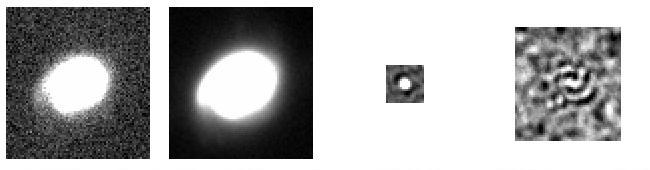
\includegraphics[height=40mm]{figures/conv_crop.jpg}
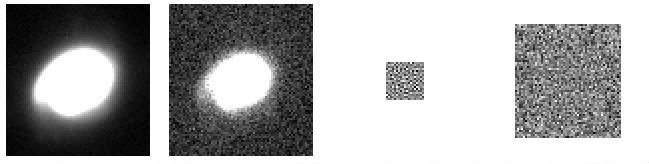
\includegraphics[height=39mm]{figures/dconv_crop.jpg}
\caption{Convolution vs. Deconvolution: The inputs and outputs
from the \code{Kernel} Model I process for a single \code{Footprint}.
For each row, we show from left to right the image that was operated
on, the image it was matched to, the derived \code{Kernel} Model I,
and the associated difference image.  In the top row, we operate on
the noisy science image, yielding a compact \textit{convolution}
\code{Kernel}.  In the bottom row, we operate on the template image 
which has a broader PSF, yielding a \textit{deconvolution}
\code{Kernel}.}
\label{fig-conv}
\end{figure}

Another way to contrast the processes is to look at a histogram of the
residuals in the difference images after the \code{Kernel} Model I
process.  Ideally, the histogram of normalized residuals will be a
normal distribution with a mean of 1.0 and root-mean-square of 1.0.
\Fig{fig-conv-stats} shows these data for the process of
convolving the science image on the left, and deconvolving the
template image on the right.  Each panel shows the histogram of all
\code{Footprint} residuals from a subset of the DC2 images, along with
the idealized normal distribution plotted as a line.  As alluded to
above, the noise distribution on the left has ``heavy tails'', 
which will lead to more spurious high-sigma
detections.  The upshot is that the spatial variation of the
convolution \code{Kernel}s may be compactly modeled.  The figure on
the right shows that the noise is better behaved when operating on the
template images.  However, the method we have chosen to model the
spatial variation of deconvolution \code{Kernel}s for DC2 appears to
fail.

% NOTE TO EDITOR : 
% CAN YOU GET THESE TO LINE UP LEFT TO RIGHT?
% RHL: They are.  What's the problem?
% ACB: I can't see how they turn out since my pdflatex is broken.
\begin{figure}[htbp]
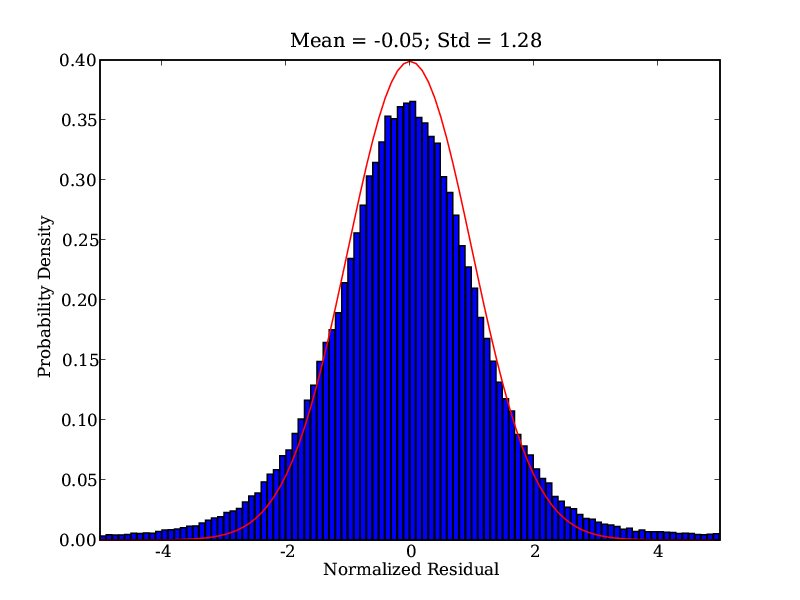
\includegraphics[height=60mm]{figures/sig30Sall.jpg}
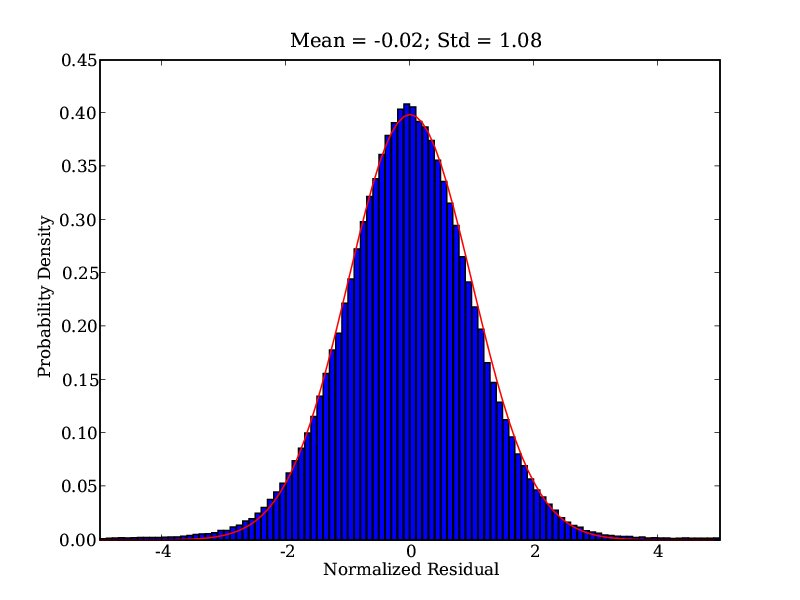
\includegraphics[height=60mm]{figures/sig30all.jpg}
\caption{Histogram of difference image pixel residuals normalized by 
the propagated noise, taken from all \code{Footprint}s after the
\code{Kernel} Model I process.  We plot the idealized normal
distribution as a solid line.  The histogram on the left shows the
results when operating on the science image, resulting in convolution.
The noise is clearly greater than expected.  The histogram on the right shows
the results when operating on the template image, resulting in
deconvolution.  The distribution is much closer to the expected normal
distribution.}
\label{fig-conv-stats}
\end{figure}

\subsubsection{Timing}

The baseline computation estimate for Image Subtraction 
%NOTE:  need reference to document that contains this
is $4.6 \times
10^{-8}$ THz--sec pixel$^{-1}$.  For DC2, we realized a speed of $2.2
\times 10^{-7}$ THz--sec pixel$^{-1}$ with both \code{fw} and
\code{imageproc} compiled with \code{opt=2}.  This is 20\% of the 
required performance.  There are 3 main sections of code that
contribute significantly to the run time: the process of accessing
pixel data; the process of convolving; and the process of filling and
inverting matrices.  The latter two depend implicitly on the first,
each requiring $\code{Footprint}_{\rm Nrow} \times
\code{Footprint}_{\rm Ncol} \times
\code{Kernel}_{\rm Nrow} \times \code{Kernel}_{\rm Ncol}$ pixel 
accesses, making this an important piece of the code to optimize.

%Pixel data are accessed through \code{fw::MaskedPixelAccessors}, which
%in turn call Vision Workbench's
%\code{vw::MemoryStridingPixelAccessor}.  {\bf RUSS - anything to say here?}.

The inverting of matrices is currently done using the \code{vw::math}
interface to \code{LAPACK}.  We are using the \code{pseudoinverse}
functionality to make the inversions more robust.  However, the
computation scaling is more severe for this process than for the less
robust \code{inverse} process.  The scaling for \code{inverse} is
$(\code{Kernel}_{\rm Nrow} \times \code{Kernel}_{\rm Ncol})^2$, while
the \code{pseudoinverse} scales to the 3$^{rd}$ power.  It is thus
important to choose the correct dimensions for our
\code{Kernel}s.  We need them large enough to represent the 
differences in the PSFs, but if we make them too large the above
scaling will start to dominate the computational budget.  There is the
additional complication that as we make the \code{Kernel}s larger, we
need to grow the \code{Footprint}s larger so that there are enough
constraints on the \code{Kernel}; their sizes are intimately
connected.  Current surveys scale the sizes using the image FWHM to
moderate the trade-off between accuracy and speed.

We should also investigate other numerical backends to undertake these
linear algebra operations, including other implementations of BLAS
(e.g.~ATLAS or Goto).  Its unclear if the current \code{LAPACK}
libraries were compiled with optimization; if not, we should realize a
significant speed-up in this processing.

\subsubsection{Issues and Lessons Learned}

The implementation of Image Subtraction for DC2 was very successful,
including stressing the build system with practical software
development, developing framework classes for pixel-level analysis
and linear algebra, and turning the process of image subtraction into
a functional \code{Pipeline}.  However, there remain several
outstanding issues, discussed above, which need to be resolved before
nightly LSST operations.  Many of these will continue on as research
and development tasks during DC3.

\begin{itemize}

\item Regularize \code{Kernel} I. This would have the advantage of 
   damping the noise in the wings of the \code{Kernel} and otherwise
   enforcing smoothness.  However, we would have to be particularly
   careful if the \code{Kernel} needs off-center power (e.g.~to
   compensate for misregistration).  Such smoothing would be
   undesirable for deconvolution \code{Kernel}s.

\item Change the order of \code{Functions}. The software needs to 
   know when there are/are not enough constraints for a given order
   \code{Function}, increasing or decreasing the order of the
   \code{Function} accordingly.

\item Do additional characterization of difference image. This includes 
   detecting and characterizing dipole residuals.

\item Enforce constraint on \code{Kernel} sum. We expect that 
   this number, representing the photometric rescaling, should be
   constant across an entire image but do not enforce this yet.

\item Have more intelligent rejection/retention of \code{Footprint}s.  We 
   will want to make sure that we have constraints for our spatially
   varying \code{Functions} across the entire image, especially in the
   corners.

\item Optimize the size of the \code{Footprint}s and 
   \code{Kernel}s. This includes taking into account the PSF
   full-width-half-maximum and crowding conditions.  In sparse
   fields, \code{Footprint}s that are too large do not add any
   additional constraints on the \code{Kernel} while significantly
   slowing down the processing.  Also, the \code{Kernel} size should
   be larger for poorer seeing data.

\item Consider circular \code{Kernel}s. This would reduce the number of 
   pixels we need for convolution operations by a factor of $\pi$/4,
   although at the cost of extra, possibly expensive, book-keeping.

\item Speed up the code. This includes optimizing convolution, finding 
   more efficient means to address image pixels, and selecting and
   optimizing the compilation of our linear algebra libraries.

\item Improve the spatial \code{Kernel} and background model. We 
   are currently using polynomial functions which can be poorly
   behaved in regions where they are not well constrained.  Options
   include using Chebyshev polynomials.

\item Explore the trade-offs between convolution 
   and deconvolution, and between operating on the science and
   template images.

\item Investigate how to compactly model a spatially varying 
   deconvolution \code{Kernel}.

\end{itemize}
